%--------------------
% Packages
% -------------------
\documentclass[11pt,a4paper]{article}
\usepackage[utf8x]{inputenc}
\usepackage[T1]{fontenc}
\usepackage{mathptmx} % Use Times Font

\usepackage[pdftex]{graphicx} % Required for including pictures
\usepackage[pdftex,linkcolor=black,pdfborder={0 0 0}]{hyperref} % Format links for pdf
\usepackage{calc} % To reset the counter in the document after title page
\usepackage{enumitem} % Includes lists
\usepackage{csquotes} % Exercise as quotes
\usepackage{amsmath} % For using "equation*" 
\usepackage{nicefrac} % For in-line fractions

\setcounter{equation}{0}% How to reset equation counter

\frenchspacing % No double spacing between sentences
\linespread{1.2} % Set linespace
\usepackage[a4paper, lmargin=0.1666\paperwidth, rmargin=0.1666\paperwidth, tmargin=0.1111\paperheight, bmargin=0.1111\paperheight]{geometry} %margins
%\usepackage{parskip}

\usepackage[all]{nowidow} % Tries to remove widows
\usepackage[protrusion=true,expansion=true]{microtype} % Improves typography, load after fontpackage is selected



%-----------------------
% Set pdf information and add title, fill in the fields
%-----------------------
\hypersetup{ 	
pdfsubject = {Nano-Optics},
pdftitle = {Assignment 1},
pdfauthor = {Vlad Tkachuk}
}

%-----------------------
% Begin document
%-----------------------
\begin{document} 

\section{Theory}
\subsection*{Exercise 1}
\begin{displayquote}
\textbf{a.}~Using the Maxwell equations, derive the wave equation for the magnetic field, \textbf{\textit{H}}, first for a general medium.
\end{displayquote}

Ampere's law describes how magnetic fields originate from electric current:
\begin{equation}
\nabla\times\textbf{H}=\frac{\partial\textbf{D}}{\partial{}t}+\textbf{J}
\end{equation}
Akin to one method of deriving Helmholz equation from Faraday's law, we can compute curl of (1):
\begin{equation}
\nabla\times(\nabla\times\textbf{H})=\nabla\times(\frac{\partial\textbf{D}}{\partial{}t}+\textbf{J})
\end{equation}
The accompanying material equation for the dielectric flux: $\textbf{D}=\epsilon_0\textbf{E}+\textbf{P}$. The electric field has a property, according to Faraday's law:
\begin{equation*}
    \nabla\times\textbf{E}=-\frac{\partial\textbf{B}}{\partial{t}}
\end{equation*}
where accompanying material equation for the magnetic flux in (3) is $\textbf{B}=\mu_0\textbf{H}+\textbf{M}$. 

Distributing the curl operator, collecting \textbf{H} in the left side of the equation, and taking the constants out yields:

\begin{equation}
 \nabla\times(\nabla\times\textbf{H})+\epsilon_0\mu_0\frac{\partial^2\textbf{H}}{\partial{t^2}}=-\epsilon_0\mu_0\frac{\partial^2\textbf{M}}{\partial{t^2}}+\nabla\times\frac{\partial\textbf{P}}{\partial{t}}+\nabla\times\textbf{J}
  \end{equation}


\begin{displayquote}
\textbf{b.}~And then use the necessary simplifications for the case of an isotropic, linear, homogeneous, nonmagnetic, medium, with no external currents and these properties do not change with time. Simplify the equation to the case of propagation through a simple optical material (eg. Silica, SiO2). Indicate how you used those approximations to simplify the equation.
\end{displayquote}
Starting from the left of the equation (2), can be simplified using a property that $\nabla\times(\nabla\times\textbf{H})=\nabla{}(\nabla\cdot\textbf{H})-\nabla^2\textbf{H}$ and noting that, in homogeneous medium, $\nabla\cdot\textbf{H}=0$. Assuming linear, homogeneous medium, $\epsilon=\epsilon_0{}\epsilon_r=const.$ and most optical materials have $\mu=\mu_0$. For dielectric non-magnetic media,  with no free charges and currents due to free charges, such as silicon oxide, $\textbf{M}=0$ and $\textbf{J}=0$. All these simplify the wave equation to:
\begin{equation}
    \nabla^2\textbf{H}-\epsilon\mu_0\frac{\partial^2\textbf{H}}{\partial{t}}=0
\end{equation}

\begin{displayquote}
    \textbf{c.} Are those approximations realistic? Give an example of such a medium. 
\end{displayquote}

These approximations are realistic in simple optical media, assuming the wavelength of the source of the electromagnetic waves is chosen to be in the transparency region of the material. Further assumptions can be made to justify them, for example, considering the dimensions of the medium of propagation larger than wavelength, absence of structural material irregularities and its perfect homogeneity. An example of such material would be the different sorts of glass used for the conventional lenses.    

\begin{displayquote}
    \textbf{d.} Give an example of media for which those approximations would not be valid.
\end{displayquote}

Any media which do not satisfy the aforementioned criteria will not be approximated. Such are the structures smaller than wavelength, like nanoscale waveguides, irregular structures like photonic crystals, anisotropic materials like those used in polarizing crystals and waveplates.

\subsection*{Exercise 2}
\setcounter{equation}{0}
\begin{displayquote}
   \textbf{a.}  Describe what a “monochromatic” wave is. What is the “bandwidth” of an ideal monochromatic wave?
\end{displayquote}

A wave which carries only one frequency and has one associated wavelength is monochromatic. Therefore its bandwidth is zero. 

\begin{displayquote}
    \textbf{b.} Do “monochromatic” waves exist in the real world?
\end{displayquote}

No, because the monochromatic waves are a mathematical abstraction. Not even spectrally pure atomic sources can radiate monochromatic waves.

\begin{displayquote}
    \textbf{c.} How would you deal with “non-monochromatic” waves in the framework of the frequency domain Maxwell equations?
\end{displayquote}
The superposition principle of harmonic functions and the linearity of Maxwell's equations allow decomposition of the input signal into the monochromatic waves and subsequent summation of the associated solutions to produce the final answer. The Fourier transform is used for this purpose.  

\begin{displayquote}
    \textbf{d.} What is the velocity at which a pulse of a certain bandwidth travels in a dispersive medium? And in a non-dispersive medium? Draw a $\omega$ − k dispersion diagram showing these two cases.
\end{displayquote}

Consider wave equation in general form for non-dispersive medium:

\begin{equation}
    \frac{\partial^2{\psi}}{\partial{t^2}}=v^2\frac{\partial^2{\psi}}{\partial{x^2}}
\end{equation}

where we can define $\nicefrac{\omega}{k}=v_p=const.$, a linear function for sinusoidal input signal of the form $A{}sin(kx-\omega{}t)$. This signal would propagate in unchanged shape as time progresses. Hence $v_g=v_p$. If we then consider a dispersive medium, for which the wave equation would become, in the simplest case:

\begin{equation}
    \frac{\partial^2{\psi}}{\partial{t^2}}=v^2(\frac{\partial^2{\psi}}{\partial{x^2}}-\alpha\frac{\partial^4\psi}{\partial{x^4}})
\end{equation}

there would be certain relation in form of $\nicefrac{\omega}{k}=v\sqrt{1+\alpha{k^2}}$ for the same input signal. Hence the group velocity is not equal to the phase velocity, and it depends on the wavelength. 

\begin{displayquote}
    \textbf{e.} Draw a dispersion diagram showing a case in which a pulse will travel very slowly. And with negative group velocity?
\end{displayquote}

If we consider an amplitude-modulated signal (wave packet), we can see the velocity of the carrier corresponds to the phase velocity, $v_p=\nicefrac{k}{\omega}$, and the velocity of the envelope corresponds to the group velocity, $v_g=\nicefrac{d\omega}{dk}$. Looking back at the case of non-dispersive medium, it is apparent that there $v_g=v_p$. 

If then $\alpha<0$ in (2), for a certain dispersive medium, there are regions in which $0<v_g<v_p$,  $v_g\approx{}0$, in which a pulse would travel slowly, or $v_g<0$, negative group velocity region. 

\begin{figure}[ht]
    \centering
    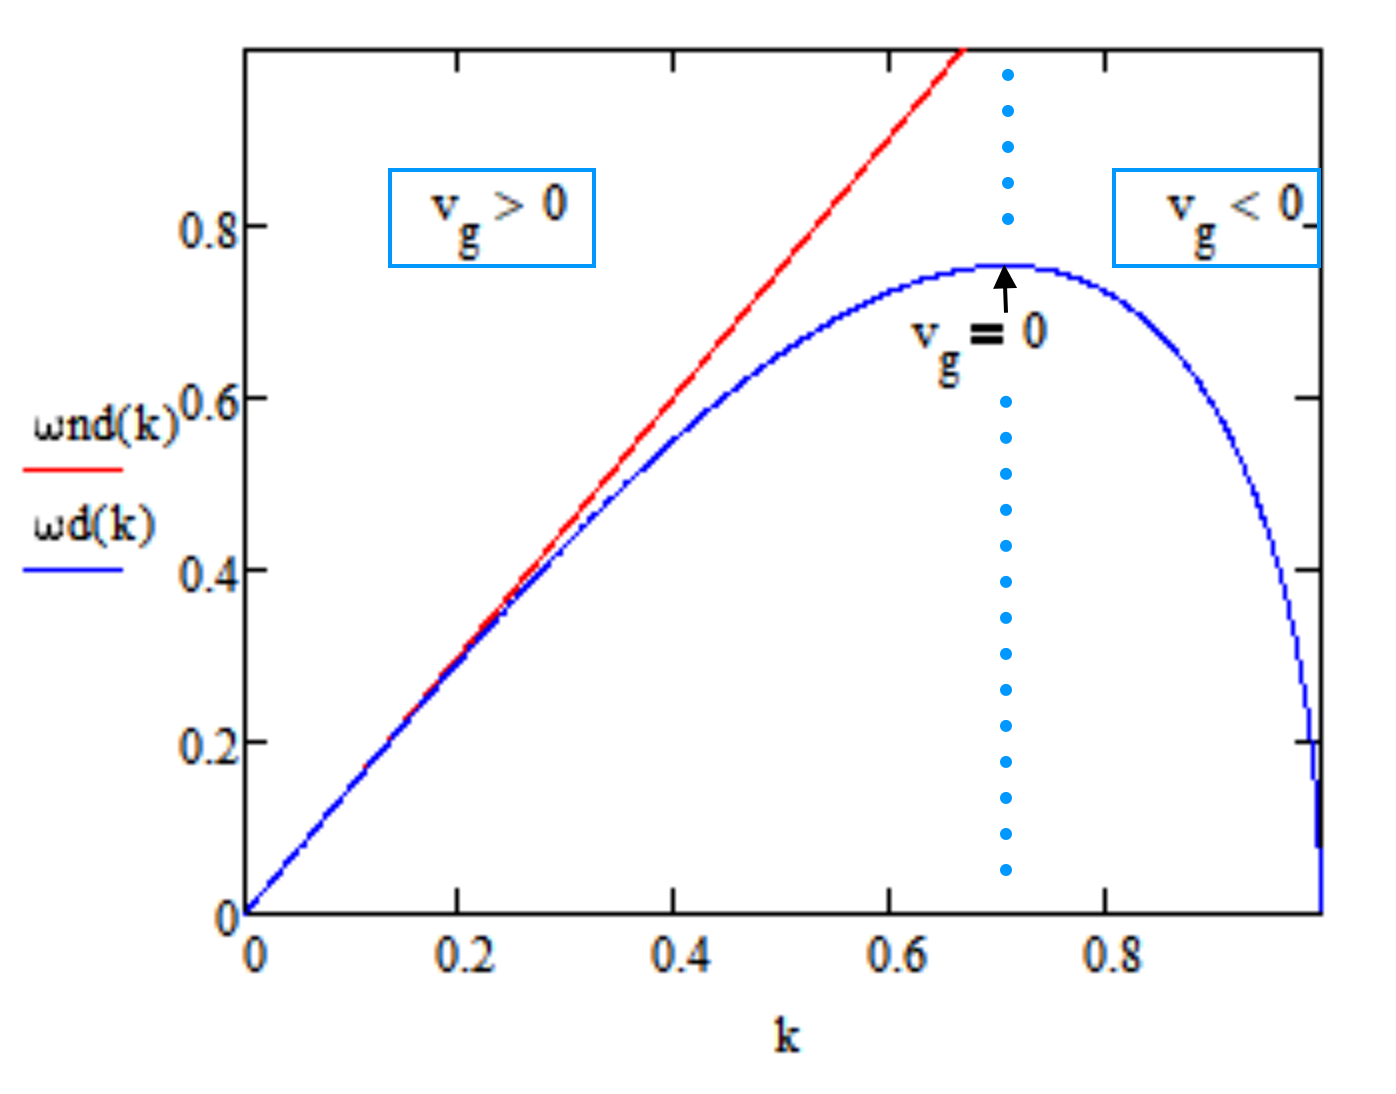
\includegraphics[width=0.5\textwidth]{ex1.png}
    \caption{Red line corresponds to dispersion relation for non-dispersive medium. Blue curve corresponds to dispersive medium. The scales are chosen arbitrarily.}
    \label{fig:my_label}
\end{figure}

\subsection*{Exercise 3}

\begin{displayquote}
    \textbf{a.} Consider a plane wave: $\textbf{E}(\textbf{r},t)=\textbf{E}_{0}e^{j(\textbf{k}\cdot\textbf{r}-\omega{}t)}$. Demonstrate $\textbf{k}\times\textbf{E}_0=\omega\mu\textbf{H}_0$.
\end{displayquote}

 Use complex notation: $\textbf{E}(\textbf{r},t)=\Re{\{\underline{\textbf{E}}(\textbf{r})e^{j\omega{}t}}\}$, such that $\underline{\textbf{E}}(\textbf{r})=\hat{x}\underline{E}_x(\textbf{r})+\hat{y}\underline{E}_y(\textbf{r})+\hat{z}\underline{E}_z(\textbf{r})$, where $\textbf{r}=\hat{x}x+\hat{y}y+\hat{z}z$, and $\textbf{k}=\hat{x}k_x+\hat{y}k_y+\hat{z}k_z$.

 Then Faraday's law in frequency domain:

 \begin{equation}
     \nabla\times\Re{\{\underline{\textbf{E}}(\textbf{r})e^{j\omega{}t}}\}=-\frac{\partial\Re{\{\underline{\textbf{B}}(\textbf{r})e^{j\omega{}t}}\}}{\partial{t}}
 \end{equation}
We can exchange the order of taking curl or partial derivative and taking the real part of a complex number. Furthermore, in frequency domain, taking a partial derivative with respect to time is equal to multiplying by $j\omega$:

\begin{equation}
    \Re{\{\nabla\times\underline{\textbf{E}}(\textbf{r})e^{j\omega{}t}\}}=\Re{\{-j\omega\underline{\textbf{B}}(\textbf{r})e^{j\omega{}t}\}}
\end{equation}

Using the definition of curl:
\begin{equation*}
    \nabla\times\underline{\textbf{E}}(r)=(\frac{\partial}{\partial{x}}\hat{x}+\frac{\partial}{\partial{y}}\hat{y}+\frac{\partial}{\partial{z}}\hat{z})\times(\hat{x}\underline{E}_x(\textbf{r})+\hat{y}\underline{E}_y(\textbf{r})+\hat{z}\underline{E}_z(\textbf{r}))
\end{equation*}
we can note that $\nabla\times\underline{\textbf{E}}(\textbf{r)}=j\textbf{k}\times\underline{\textbf{E}}(\textbf{r)}$. We know that $\underline{\textbf{B}}=\mu\underline{\textbf{H}}$. Hence:

\begin{equation}
      -j\textbf{k}\times(\underline{\textbf{E}}_{0}e^{j(\textbf{k}\cdot\textbf{r}-\omega{}t)})=-j\omega\mu\underline{\textbf{H}}(\textbf{r},t)
\end{equation}

The complex component of the magnetic field can be determined from the corresponding complex electric field, so $\textbf{H}(\textbf{r},t)=\textbf{H}_{0}e^{j(\textbf{k}\cdot\textbf{r}-\omega{}t)}$  which implies:
\begin{equation}
    \textbf{k}\times\textbf{E}_0=\omega\mu\textbf{H}_0
\end{equation}

\begin{displayquote}
    \textbf{b.} What can you comment about the meaning of this expression?
\end{displayquote}

$\underline{\textbf{E}}_0$ contains information about the polarization, amplitude and absolute phase of the wave at the origin. $e^{j\textbf{k}\cdot{\textbf{r}}}$ tells how the phase of the wave evolves with position. $\textbf{k}\cdot\textbf{r}$ is the planar phase front of propagating transverse electromagnetic wave: $\textbf{k}$, $\textbf{E}$ and $\textbf{H}$ form a right-handed orthogonal system. 

\section{Lumerical} 

\begin{figure}[ht]
        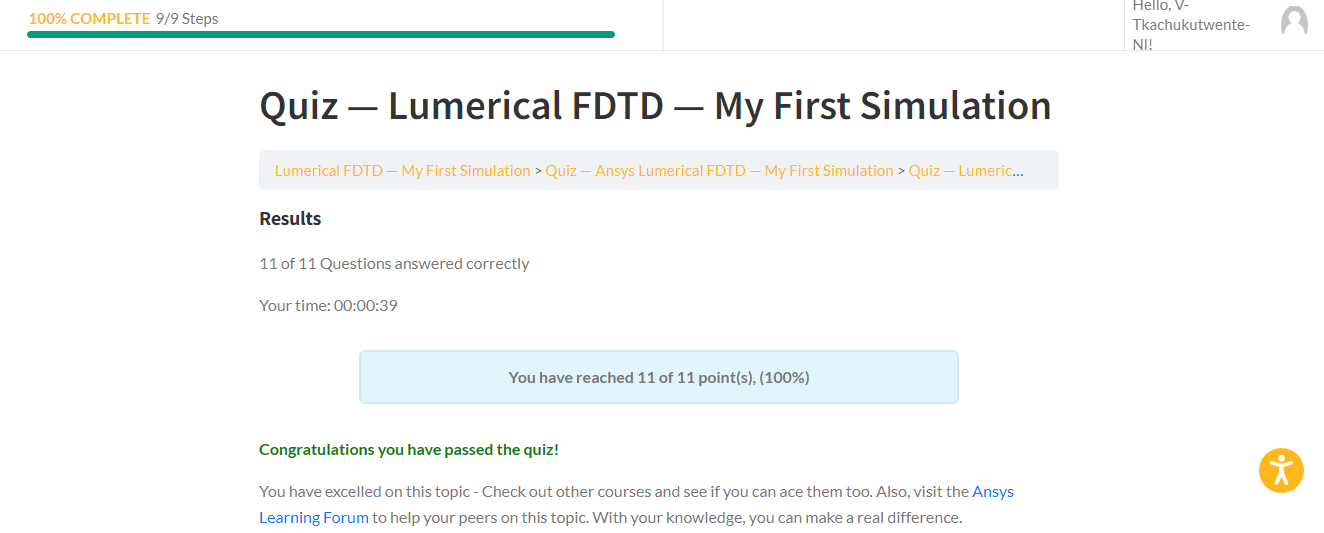
\includegraphics[width=0.95\textwidth]{fig1.png}
\end{figure}

\begin{figure}[ht]
        
\includegraphics[width=0.95\textwidth]{fig2.png}
\end{figure}

\begin{figure}[ht]
        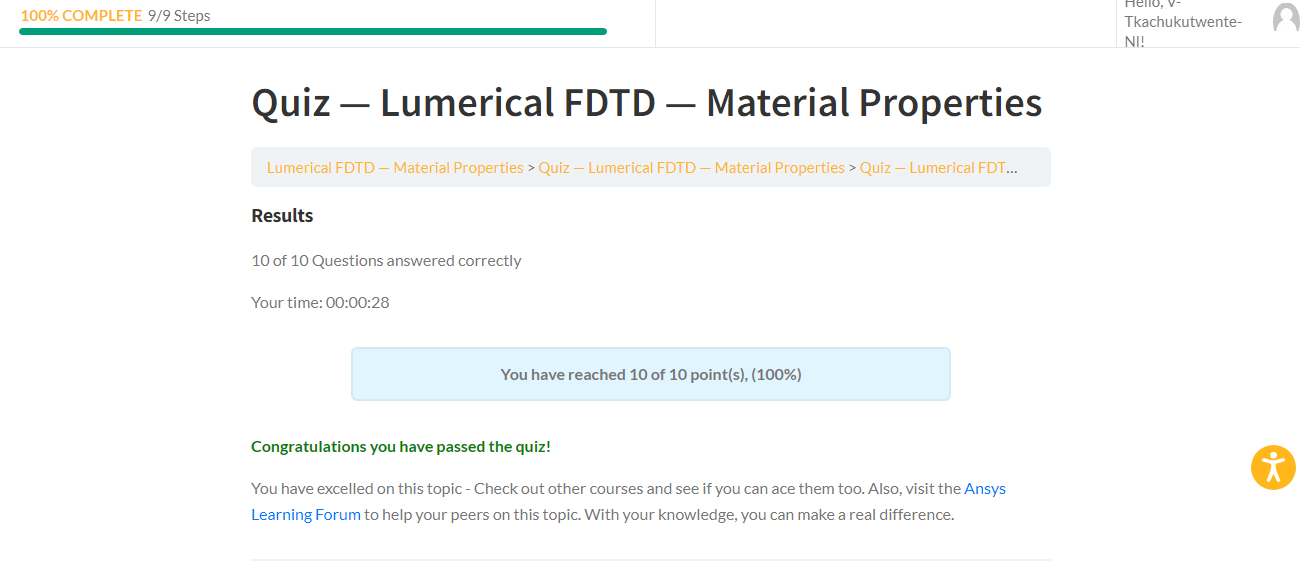
\includegraphics[width=0.95\textwidth]{fig3.png}
\end{figure}

\begin{figure}[ht]
    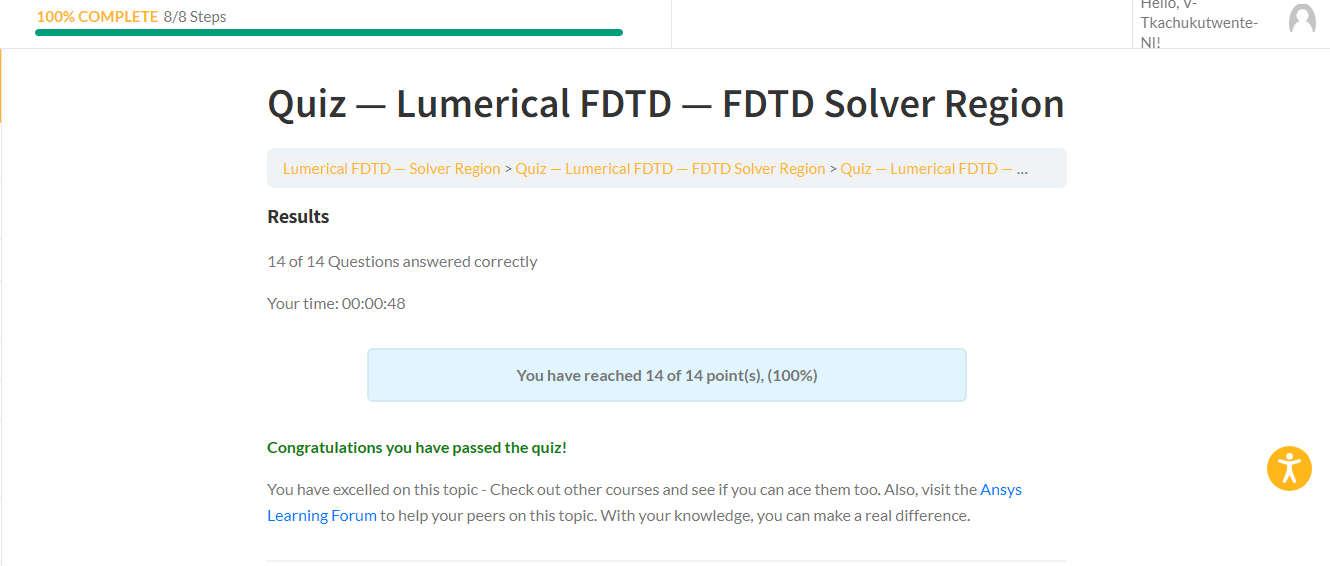
\includegraphics[width=0.95\textwidth]{fig4.png}
\end{figure}


\end{document}
